%%%%%%%%%%%%%%%%%%%%%%%%%%%%%%%%%%%%%%%%%%%%%%%%%%%%%%%%%%%%%%%%%%%%%%
%
%   File          : related_work.tex
%   Author(s)     : Ashwin Shashidharan <ashashi3@ncsu.edu> and Jitesh Shah <jhshah@ncsu.edu>
%   Description   : Related Work for the Project
%
%   Last Modified : Wed Sep 28 21:30:30 EDT 2011
%   By            :  Ashwin Shashidharan <ashashi3@ncsu.edu> and Jitesh Shah <jhshah@ncsu.edu>
%
%%%%%%%%%%%%%%%%%%%%%%%%%%%%%%%%%%%%%%%%%%%%%%%%%%%%%%%%%%%%%%%%%%%%%%

\documentclass[10pt,twocolumn,pdftex]{article}
\usepackage[margin=1in]{geometry}
\usepackage{comment}
\usepackage{ifthen}
\usepackage{graphicx}
\usepackage[hyphens]{url}
\usepackage{times}
% hyperref sometimes causes strange build errors. Comment if problems
\usepackage[pdftex,colorlinks=true,citecolor=black,filecolor=black,%
            linkcolor=black,urlcolor=black,draft]{hyperref}
%\usepackage{listings}
%\usepackage{fancyvrb}
%\usepackage{amsmath}
%\usepackage{amsthm}
%\usepackage{amssymb}

% Some quick utils
% Use:
% \begin{itemize} \itembase{3pt}
%  \item ...
% \end {itemize}
\newcommand{\itembase}[1]{\setlength{\itemsep}{#1}}

\title{Enabling Cloud Customers to Trust the Cloud}

\author{Ashwin Shashidharan and Jitesh Shah \\
\url{{ashashi3,jhshah}@ncsu.edu}
}
\date{November 30, 2011}
\begin{document}

\maketitle

\begin{abstract}
Cloud computing has emerged into a very popular \cite{adoption-survey} means of scaling up quickly without the associated infrastructure costs. The promise is complete freedom from maintaining own server infrastructures and moving to third-party infrastructure providers. Despite it's increasing popularity, a significant chunk of applications haven't yet found a place in the cloud. The reason is the lack of guarantees, from the cloud provider, about the security of customer data stored on the cloud. Even in the presence of such guarantees, the cloud customer would want to ensure that a very small chunk of \emph{auditable} infrastructure on the cloud side is trusted. Using that as a Trust Computing Base (TCB), the customer would build his own security to protect his data, thus, having the guarantees. Note that the threat to the customer data does \emph{not} come from the cloud provider, but, attacks on the cloud provider by competitors using the same cloud service or other external attackers. 

This paper proposes a way to enable the customer to protect its data in the face of a cloud compromise. Two key technologies are used to build the security architecture: SELinux (Security Enhanced Linux) \cite{SELinux} and TPM (Trusted Platform Modules) \cite{TCG}. Both of these technologies allow confining the root user. We also describe a range of feasible attacks and how the customer data can be protected in the face on these attacks using the proposed architecture.\\ \\
\emph{Keywords}:  Trusting the cloud, SELinux, TPM, SSL/TLS, symmetric encryption/integrity verification.
\end{abstract}

\section{Introduction}
According to a Berkeley publication \cite{controlling-data-in-the-cloud}, all the top five software companies by sales revenue have their own cloud offerings. Popular sites such as reddit.com and quora.com run completely off the cloud. Merrill Lynch estimates the market capitalization of the "Cloud Computing" sector to be as large as 16B in 2011. Inspite of such impressive growth, a Morgan-Stanley survey \cite{morgan-stanley} says that only 28\% respondents of the survey use public cloud of some form in their daily operations whereas only 14\% use IaaS services of any kind. Various publications \cite{controlling-data-in-the-cloud, ENISA} clearly identify the risks associated with security of the storing data in the cloud. Fear of leakage of sensitive data from the cloud is a common thread in these publications. These risks induce a "Fear of the Cloud", thus, slowing down adoption. Vulnerabilities discovered in popular cloud services like Amazon EC2 \cite{amazon-ec2-vulnerability} and Dropbox \cite{dropbox-vulnerability} exacerbates the fear. 

For corporations to offload their secure data to the cloud, they need to have guarantees against leakage of thire data. Such guarantees can come only from a huge audit of the cloud provider, which might be unfeasible and time consuming considering the size of the cloud providers, or getting themselves involved in designing of the security on the cloud provider side. The cloud can thus be viewed, from the perspective of our project, as a provider of infrastructure and a Trusted Computing Base (TCB) which can be utilized by the cloud customers to enforce a security policy. \\

Various methods have been proposed in the past to avoid data leakage from the cloud. Simply encrypting data in the cloud (without any trusted software) has been discussed in literature sparingly \cite{cryptographic-cloud-storage, towards-secure-cloud-storage}. The problem with just encrypting the data, without attestation of the underlying software, is that the underlying software could have been maliciously modified by an attacker who has broken into the cloud provider. A modified guest kernel would definitely be able to steal all the encryption keys. So, even though encryption is an essential component of securing the data, a trusted computing base is essential too.

Setting up a Trusted Computing Base (TCB) for the cloud has been more widely discussed \cite{towards-trusted-cloud-computing, seeding-clouds-with-trust-anchors, terra, semantic-remote}. A TCB is setup with an established root of trust. The root of trust is usually a TPM (Trusted Platform Module). Beginning with the TPM, the BIOS, bootloader and the Operating System are verified before passing control to them. Any modification to any of the above components would lead to failure of Remote Attestation. The problem with such an approach is that, it provides security only in static aspects. Any attack on the runtime system (process, memory, etc) would go undetected. 

Literature also talks about runtime integrity verification \cite{integrity-1, integrity-2, integrity-3, integrity-4}. The problem with runtime integrity verification is that they are very difficult to get right in practice. No cloud in the current market offers runtime integrity verification \cite{seeding-clouds-with-trust-anchors}.

Without runtime integrity protection, the data on the cloud will still be vulnerable to attacks of the dynamic nature. A practical alternative to runtime integrity verification is to sandbox the trusted VM launcher process, minimize its interaction with the outside world and audit the small external facing code thoroughly for security vulnerabilities. Thus, in addition to encryption and trusted computing, we propose to use strong Mandatory Access Control (MAC) based confinement techniques to sandbox the trusted VM launcher and the kernel images. This can be viewed as a light-weight and practical alternative to the complex runtime integrity verification techniques. SELinux \cite{SELinux} is an implementation of MAC on Linux-based systems. We use SELinux to sandbox the launcher and thus, protecting it from dynamic attacks. Hardening the core virtual infrastructure of a cloud has been discussed in atleast one paper before \cite{secure-cloud-core}. 

We propose that the cloud customer encrypt and integrity verify the kernel used to boot his VM image. Since the threat model is attack on the cloud, we propose that the keys for encryption/decryption of kernel and the data (two separate keys) be stored on the customer side. The keys are revealed only to an attested and authenticated (via SSL \cite{SSL}) cloud process. The cloud process verified cloud process then goes on to provision the guest image on one of its machines.

Note that the core of the idea is protection of business critical data in the face of attacks on the cloud infrastructure.

Section \ref{sec:background} explains some terminology used widely in the paper. Section \ref{sec:problem} further explains the problem statement and the threat model (what we protect against). Section \ref{sec:approach} explains and justifies the solution in detail. Section \ref{sec:evaluation} lists the types of possible attacks that we envision and defences in place against them. Section \ref{sec:related} lists some related work we are aware of and lastly section \ref{sec:conclusion} concludes the paper.

\section{Background}
\label{sec:background}
In this section we will give a background of some of the technologies employed in the project.

\subsection{Trusted Platform Module}
The Trusted Computing Group (TCG) \cite{TCG} was formed with a goal of creating a Trusted Platform Module (TPM). A TPM is a secure cryptoprocessor which is activated from very early in the boot process. The property of TPM which makes it useful is that it can seal data inside it and reveal only to a verified authority. Since, the data inside the TPM is unforgeable, TPM can be used as a root of trust. The idea is to start with this root and expand the perimeters of trust one-by-one from BIOS to the OS to the applications.

A TPM usually has a small processor which can do symmetric as well as asymmetric cryptography. An asymmetric key called the SRK (Storage Root Key) is burnt into the TPM, unreadable by the external world. The SRK is used to create a tree of keys used to perform encryption/decryption. This makes sure that any encrypt/decrypt operation needs SRK and hence, an involvement of the TPM.

There is also some permanent storage available in the form of Platform Configuration Registers (PCRs). There can be upto 32 such PCRs according to the TCG 1.2 specification. It is not possible to directly write to a PCR. A TPM supports only two operations to a PCR: Read and Extend. Following paragraph describes how to establish trust using a TPM.

When the machine is reset, TPM is booted with all PCRs reset. The hardware then calculate the hash of the BIOS code and extends it to a PCR in the TPM, say, PCR\#16 and the control is passed to the BIOS. The BIOS calculates hash of the boot loader and extends it to PCR\#16 again and passes control to the bootloader. The bootloader does the same for the kernel. Thus, after the kernel is booted, the value in PCR\#16 is a unique summary of {BIOS, bootloader, kernel} tuple. Any modification in either of these will change the value in PCR\#16. Now keys can be created and data encrypted against PCR\#16. Only unmodified kernel can then unseal the secret values. Thus, a TPM can be used to reveal secrets only to trusted parties. 

Note that to perform these operations on a TPM, AuthData is required. AuthData can be thought of as the key to unlock the operations of the TPM. It could be as simple as a password or a complex derivation (salted hash, etc) of a password. 

\subsection{SELinux}
\label{sec:selinux}
Security Enhanced Linux (SELinux) \cite{SELinux} is an implementation of Mandatory Access Control (MAC) over a traditionally DAC (Discretionary Access Control) implementation on Linux Systems. The advantage of MAC over DAC is that the security policy is centrally administered from a policy database and cannot be modified by the users. MAC also offers a more fine-grained control on the resources that can be accessed by a subject. For example, it is possible to disallow Apache httpd to send emails, but allow to write files in a certain directory.

SELinux bases it decisions on the tuple {user, role, type}. The user is SELinux user and \emph{not} the Linux user. Roles can be used to implement RBAC (Role Based Access Control). Type is field on which access control decisions are based on. This 3-tuple is known as the \emph{context}. Each subject and object has a context. To execute a file from a different context, a transition rule must explicitly enable the process to transition from one context to the other. Execution then continues on the new context. Read and write accesses can be granted to other types. For example,\\
{\tt \# allow user\_t other\_t:file create \{read\}} \\
The rule states that \emph{user\_t} type is allowed to only read the files on the type \emph{other\_t}.\\

We use SELinux to sandbox the launcher process and to confine the root user.

\subsection{SSL/TLS}
Transport Layer Security or its predecessor Secure Socket Layer is a cryptographic suite used to provide encrypted and authenticated communication between two parties who trust a thrid-party called the Certificate Authority (CA). SSL/TLS is now being widely deployed on all major websites including Google, Facebook, Twitter, etc to avoid several man-in-the-middle and DNS attacks. 

We use SSL/TLS to mutually authenticate the cloud provider and the customer site. We also use encrypted communication to transfer sensitive data from customer site to the cloud side.

\subsection{Miscellaneous}
This subsection will explain terminology used throughout the paper.
We use the term \emph{Management node} to refer to a node in the cloud which is exposed to the outside world as well as the VM image store, which makes it vulnerable to attacks. The term \emph{Launcher} is used to denote the process which launches and provisions the guest image upon a trigger from another process (like the webserver. The webserver accepts launch requests from the customer and triggers the \emph{launcher}). 

\section{Problem Statement}
Our work deals with securing the process of image loading that is done by the management node and protecting against tamper of images in the image library. All assumptions about the cloud architecture are based on our study of VCL. We begin by briefly explaining the VCL architecture and following it up with threats and risks in this setup.

\subsection{VCL Architecture}
The VCL cloud architecture \cite{vcl-arch} associates resources in the cloud with different levels of abstraction. Applications are associated with the use of custom images and OSes that run on hypervisors. While computing and hardware resources are handled by the use of a VCL Manager Software, network resources are managed by the use of virtual networks, VLANs and VPNs.

The VCL Manager Software runs on a management node that is responsible for hardware resource allocation, provisioning, optimal scheduling, launching and scheduling image instances. User requests are mapped by the VCL Manager software onto available software application images and available hardware resources. It is then scheduled for use by the customer.

The VCL node manager handles both bare-metal images, that run directly over a machine and virtual images that run on a hypervisor. It is imperative to know that, the management node has three interfaces that it uses to load images, connect to the management module on a chassis, and for incoming connections from the public network. The VCL architecture has been illustrated in Figure 1.\\

\begin{figure*}[htp]
\centering
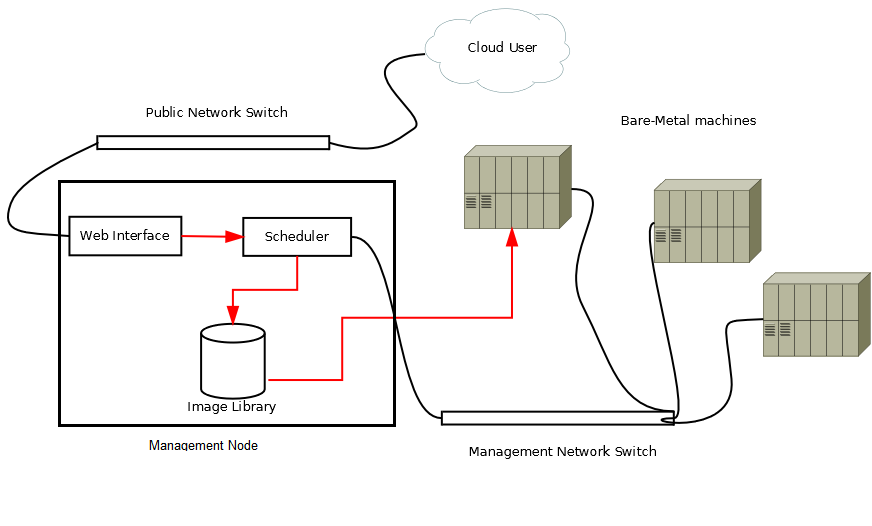
\includegraphics[scale=0.50]{csc574-vcl-architecture.png}
\caption{\small \sl NCSU VCL cloud architecture. The red lines denote the control flow in the cloud. The management node is shown connected to a public network switch for incoming public connections and a management network switch to perform administrative actions and management. }
\label{fig:solution}
\end{figure*}	

The management node is vulnerable to exploits in its OS, middleware and other software components. The management node is vulnerable owing to the fact that it accepts connection over the public network. Misconfigurations and vulnerabilities in the httpd and ssh daemon or other system software may be exploited to take control of the node. We expect the cloud provider to be resilient to such attacks and also, in the event of a compromise the user data to remain protected.
\subsection{Possible attacks}
We now describe a few attack scenarios and try to assess the magnitude of loss.

As mentioned earlier, the management node has a processing engine to process reservations obtained from the VCL web portal and access to the image library over one of its links. An adversary who has attained sufficient privileges on the management node can thus create havoc by loading images that were never requested. Access to the image store is more lethal, if the adversary has also gained modification rights for storage. If there is no mechanism in place to verify the integrity of images before a launch, the attacker may launch malicious image instances. These instances may then be used to capture user sensitive information transferred usually during a connection request. In another case, can make the image unavailable thereby launching a DoS attack. The use of a malicious modified image by the attacker can also be used to capture/manipulate data generated by those instances.

An adversary who has gained access of the management node may also tamper with out-of-band management features, central to proper functioning of the infrastructure itself. With control features enabled for bare-metal machines and images, from the management node, an adversary gains access to all these resources on a compromise

The management node also has total control over bare-metal machines and virtual machines that it has launched. Root access to the attacker on the management node further can be used to take control of these bare-metal machines.

The management node is also responsible for provisioning and scheduling, on a compromise, the attacker can use the computing power available on the cloud to launch attacks on other instances running in the cloud.
Access to the data store is another concern. In the event of a storage compromise, without encryption to protect the confidentiality of user data, user's data on the cloud becomes accessible to the attacker.

Thus, we conclude that the management node is central in a cloud setup to manage user requests, schedule resources, security and multi-site coordination.

We expect most of the cloud environments to have such a node and through our design and implementation we have provided in this paper, we secure the cloud's management node from static attacks that tries to launch altered components in an expected flow of execution. We try to address the problem of being able to use the cloud with an assurance of security and devise a solution whereby, the customer is also made part of this process.\\\\
In the next section we describe how we take on the above challenges.

\label{sec:problem}

\section{Approach}
\label{sec:approach}
As we saw in the last section, obtaining root access on the Management node can be catastrophic. It is never possible to claim with a 100\% guarantee that a particular software is free of bugs. Thus, putting in measures to check the damage in case of a compromise is as necessary as following secure coding practices. The next subsection attempts to summarize the salient points of the design. 

\subsection{Design Choices}

\subsubsection{Store keys on customer site}
The fundamental premise of the project is to enable the customer to trust the cloud. Thus, we choose to store the data and kernel encryption/decryption keys on the customer site. The customer site reveals the keys only to a \emph{secure launcher daemon} on the cloud side, who can attest its state and authenticate via SSL. (Note: Workings of the \emph{secure launcher daemon} is discussed in the later section)

\subsubsection{Integrity check the kernel}
The kernel which the guest VM uses to boot should run unmodified. Any malicious alteration in the kernel can lead to leakage of data. Thus, the customer site stores an HMAC of the kernel alongwith the kernel decryption key. This, HMAC is passed along to the \emph{secure launcher daemon}. Only if this HMAC matches the one obtained from the kernel, is the kernel booted. Note that we also store the kernel encrypted on the cloud side (although one might argue that it isn't really necessary).

\subsubsection{SSL private key a sealed by the TPM}
To enable mutual authentication between the cloud provider and the customer site, they communicate via SSL. If an attacker has to pose as the cloud provider, he will need the SSL private key of the cloud provider. To avoid imposters, we seal the SSL private key in the TPM. This private key can now only be accessed if the TCB established and the \emph{secure launcher daemon} is unmodified.

\subsubsection{TPM Authdata management}
To perform a TPM seal/unseal operation, it is necessary for the requesting entity to show Authdata: an entry ticket into the TPM. Authdata can be as simple as passwords or a complex derivation of passwords. We let the cloud customer choose the Authdata type. The Authdata can either be entered manually on a terminal when launching a guest VM, can be passed on from the customer site with the launch request or can be stored in a file with very strict SELinux confinements. The most preferable and secure way is to enter it manually on the terminal (might not be the most practical). 
\\

Next we provide an overview of how the solution works.

\begin{figure*}[htp]
\centering
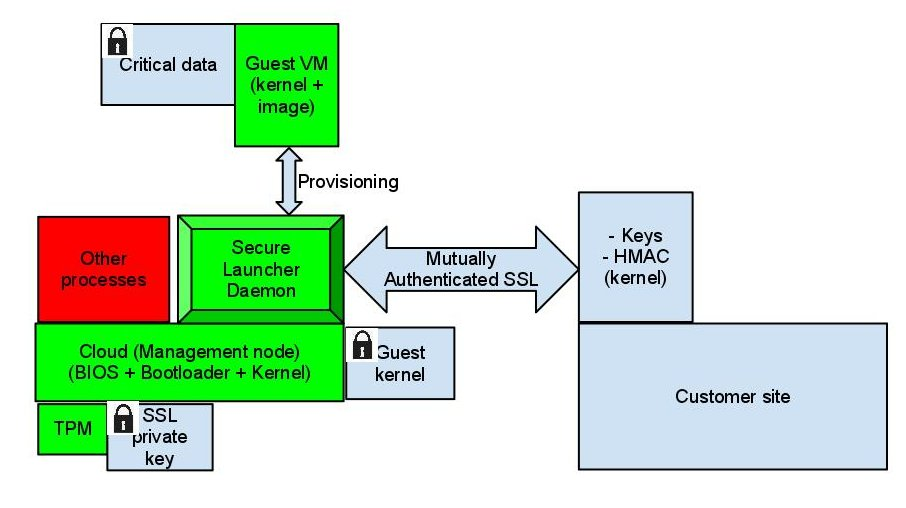
\includegraphics[scale=0.50]{csc574-solution.jpg}
\caption{\small \sl The architecture of the solution. The green parts denote trusted entities. Red denotes entities not in the TCB. The SSL private key is shown near the TPM block to signify that it is sealed in the TPM. The locked entities can only be unlocked by the trusted Secure Launcher Daemon. The guest VM resides on a different node. }
\label{fig:solution}
\end{figure*}
\subsection{Initial Setup}
For the success of this scheme, customer's participation is required in setting up the initial security of the system. In this section, we cover how the initial setup is done.

The customer first sets up separate keys for encryption/decryption of the kernel and the data. The cloud provider either sends a copy of the kernel to be authenticated by the customer or the customer compiles his own copy. In the former case, the unencrypted kernel is sent via snail-mail on a harddrive with proper digital signature. The customer verifies the digital signature, creates an HMAC with his kernel signing key and encrypts the kernel. The encrypted kernel is then returned via snail-mail, again, with proper digital signature. The customer keeps the HMAC. The cloud provider installs this encrypted kernel on his side. Note that the snail-mail is only to provide a secure out-of-band communication mechanism.

The customer then sets up an SSL-enabled server to serve the keys and the HMAC to properly authenticated cloud entity. 

On the cloud side, the customer takes part in setting up the TCB. The customer can, optionally, provide a TPM. The TPM setup procedure is fully audited by the customer to ensure security (Core assumption is that the cloud provider is trusted and the setup procedure won't be botched. The audit is to make sure that the proper security policies are adhered to). The setup of the management node occurs behind closed doors with no access to the external world, so it is assumed that it cannot be compromised by an external entity.

A proper hash of {BIOS, bootloader, kernel, secure launcher daemon} is extended in on the PCRs of the TPM. The SSL private key of the cloud used for authentication with the customer is then sealed off againt the said PCR. Proper SELinux policies are then put in place to sandbox the secure launcher daemon.

The next section describes the operation of the setup.

\subsection{Solution}
The very first step to secure data in the cloud is to encrypt it. The cloud provider can provide facilities for encryption just before storing to the persistent storage at the cloud site. However, according to the end-to-end argument \cite{end-to-end}, if the cloud customer needs guarantees, the encryption has to be done at the application layer by the customer software. The customer may choose to have a full-disk encryption (encrypts the whole filesystem) \cite{disk-encryption, truecrypt} or a selective file-encryption \cite{nss}. In either method, for efficiency reasons, the encryption technique chosen would probably be some kind of symmetric encryption (like AES) and will need a key. 

This key cannot be stored on the guest image in plaintext, since the attacker has access to the guest image from the management node and he can directly read it off the image. As describer above, the keys will be revealed only to a cloud process who can provide attestation (using TCB) and authenticate itself using SSL. Next we describe ways in which it will be impossible (or atleast hard) for an attacker to falsely pose to the customer as an attested cloud process.

Now refer to Figure \ref{fig:solution} for an overview of the architecture.
A TPM is used to establish a TCB, as we saw in the "Background" section. The TPM verifies the BIOS, bootloader and the kernel. Eventually, the kernel extends the hash of a \emph{secure launcher daemon} in the TPM and starts the daemon. The job of this daemon is to listen for requests to launch a VM. When a request is received, it unseals the SSL private key from the TPM. This unseal operation only works if neither of the BIOS, bootloader, kernel or secure launch daemon have been modified.

After the SSL private key is unsealed, the daemon can authenticate to the customer site. Once the customer site authenticates the cloud provider, it releases the following objects: kernel decryption key, data decryption key and an HMAC of the kernel image.

The \emph{secure launcher daemon} decrypts and verifies the integrity of the kernel. It then reads the actual launcher binary (usually a provisioning engine like xCAT \cite{xCAT}) into memory, calculates its hash and compares against the expected hash. If both the kernel and the launcher binary are verified, then the daemon forks of the launcher process which does the appropriate provisioning.

The data decryption keys are passed on to the guest kernel via a shared page or as a provisioning parameter.

Note that the \emph{secure launcher daemon} is confined using SELinux. The SELinux policy recommendations and how to sandbox the daemon is described in detail in a later section.

\subsection{SELinux Policy}
An introduction to SELinux can be found in section \ref{sec:selinux}. Confining the secure launcher daemon to a sandbox is a critical part of protecting the data. The SELinux policy should be able to protect the sandboxed daemon from the following intrusions: Compromised server (httpd, sshd, etc) giving root access to the attacker and password guessed for one of the users for sshd eventually giving root access on the management node to the attacker. 

Before discussing the SELinux policy, it would be worthwhile to discuss some SELinux quirks.

Three SELinux usertypes we need to know about are: {\tt user\_u, system\_u and unconfined\_u}. The {\tt user\_u} type is the most restrictive among the three. It allows the user only to access files which are allowed to the {\tt user\_t} type and the types it can transition to. The user type {\tt system\_u} is reserved for system operations and SELinux commands. The {\tt unconfined\_u} user is a special user category which reduces the user to the DAC privileges i.e. no MAC. Clearly, {\tt unconfined\_u} and {\tt system\_u} user types are potential threats to the security of the system and need to be well-monitored.\\

A management node on the cloud has a defined set of responsibilities and hence, known set of software running on it with known responsibilities. This makes it feasible to write \emph{strong} SELinux policies for it. Each server/daemon should be constrained to its own domain and given access to just the files it absolutely needs. This is not an unruly demand. Fedora already comes with a Targeted SELinux policy that has known servers (httpd, sshd, etc) appropriately confined. For example, httpd subjects and objects are labelled with the type {\tt httpd\_t}. 

Writing a new policy from scratch for the Management node is a tough job. One needs to know a lot about the internal workings of a program to be able to write a policy for it. Consequently, a better approach is to start with a stock policy like Fedora's targeted policy and rip-off the potentially insecure parts.

The targeted policy maps each Linux user to the SELinux {\tt unconfined\_u} user. As we have seen above, such a mapping reduces the system to a DAC system. This gives the root user ultimate privileges. In order to confine root, it is necessary to remove the {\tt unconfined\_u} SELinux user totally from the system. This can be done by the following set of commands:\\ \\
{\tt \# sudo semanage login -m -s "user\_u" -r s0 \_\_default\_\_}\\
{\tt \# sudo semanage login -m -s "user\_u" -r s0 root} \\
{\tt \# sudo semodule -r unconfined}\\

The first command maps all the Linux usernames to {\tt user\_u} SELinux user. The second command maps the Linux root user to {\tt user\_u} SELinux user.  The third command removes the unconfined module. Removing the unconfined module greatly adds to the security. The Linux root user can now be confined and hence, damage control is possible.

\subsubsection{Sandboxing the secure launcher daemon}
A new SELinux user is now defined for secure launcher daemon, say, {\tt secure\_u}. All the files needed by the daemon are marked with the type {\tt secure\_t}. Thus, only the secure daemon can access the files. No transition is allowed to or from {\tt secure\_t} type. This gives the appropriate sandboxing. 

\subsubsection{Constraining the root user}
Mapping the Linux root user to the SELinux {\tt user\_u} user already took off many of the privileges of the root user. Adding "PermitRootLogin=no" to the sshd config disallows root login over ssh. But, it would be truly wishful thinking to assume that a root login will never be needed. Upgrading the guest machine, Adding new software, Reconfiguration would be impossible without root. The trick then is to permit a transition to the unconfined domain ONLY if the user can prove physical access. Physical access means the process should have a tty. Adding the following line to the {\tt /etc/sudoers} will enable one to sudo to root user with unconfined access: \\

{\tt root ALL=(ALL) TYPE=unconfined\_t ROLE=unconfined\_r ALL} \\

A minor patch to "sudo" will check for the presence of tty (using a call to {\tt isatty()}) before granting the root access. 

Since a remote attacker can never have a physical tty, he can never have an unconfined root access to the management node.

\section{Experimental Evaluation}
\label{sec:evaluation}

\subsection{Tools Used}
Since none of us had access to a real TPM, we used a TPM emulator software from BerliOS ({\tt tpm\_emulator-0.7.2}). It exports a device {\tt /dev/tpm} and a user-space daemon {\tt tpmd} which emulates the TPM hardware. Any requests on the TPM device file are forwarded to the daemon for execution. We used the {\tt TrouSerS} library to interface with the TPM in userspace ({\tt trousers-0.3.6}). We also used a patched version of {\tt tpm-tools-1.3.5} package for the TPM unseal operation.

We used the {\tt OpenSSL} library for SSL communication and symmetric key encryption/decryption/integrity verification. Specifically {\tt openssl-1.0.0e-1}. 

Since actual implementation of a cloud with a provisioning engine is infeasible on a local machine, we used a poor man's cloud: a virtual machine. We chose KVM \cite{KVM}, since it is popular and opensource. Overall to come up with a proof of concept, we used the following tools: Host machine acts as Management node. {\tt qemu-kvm} acts as the provisioning engine (It is actually an emulator, but at a higher level, given a kernel image, it first does the appropriate provisioning on the host machine and then boots the image). Specifically we used {\tt qemu-kvm-0.14.0} as our "launcher". \\

All the experiments were performed on a Lenovo SL510 laptop running a Core 2 Duo @ 2.1GHz processor with 1GB of RAM. 

\subsection{Attack Vectors}
In this section we describe the various attacks that an attacker can launch and our defences against them. The premise of an attack is that the attacker can obtain \emph{remote root shell access} on the management node. This may me obtained by compromising one of the servers running on the management node or guessing a password of one of the users over sshd (either root user or other non-root user). In the presence of this shell access, the problem definition is to protect the confidentiality of customer data.

\subsubsection{Re-program the TPM}
Since TPM is our root of trust, a malicious attacker can try to reset the TPM to cause DoS a attack or the attacker can try to unseal the SSL private key using PCR\#16 which already has the correct extended hash. There are two defences in place against this attack:
\begin{enumerate}
\item Authdata is required to seal/unseal data from the TPM or program the TPM.
\item The TPM device, {\tt /dev/tpm} is labelled as {\tt secure\_t} and hence, can be accessed only by processes who can transition to that type. Thus, only processes part of TCB i.e. the secure launcher daemon and the actual launcher is allowed to access the TPM device.
\end{enumerate}

\subsubsection{Steal kernel/data encryption keys}
The attacker can try to steal the kernel encryption key (to create a malicious kernel and a valid HMAC for it) or the data encryption key (to compromise the actual customer data). The defences against these attacks are:
\begin{enumerate}
\item The customer site reveals the keys only to properly attested and authenticated cloud process. To authenticate to the customer site, the attacker will need the SSL private key of the cloud provider. This has been sealed off in the TPM and can be unsealed only by processes in the TCB as explained earlier. 
\item SELinux confinements make sure that no user or server gets unconfined access to the management node. Unconfined access can only be obtained via a physical terminal. Thus, privileged operations like inserting a kernel module in the kernel are not possible for a remote attacker, thus, disallowing the attacker to sniff memory after SSL has decrypted the keys into memory.
\end{enumerate}

\subsubsection{Modify the kernel}
The attacker may try to maliciously modify the guest kernel in order to steal the customer data. However, the kernel is stored encrypted and integrity-protected. Thus, any modification in the kernel will be caught and the secure launcher daemon would refuse to boot the kernel. Also, SELinux confinements make sure that the kernel image is marked with the type {\tt secure\_t} and thus, can only be accessed by the processes in the TCB.

\subsubsection{Use a customized kernel}
The attacker may just try to get his own kernel copy and a launcher binary and try to boot an image completely outside of the TCB. Although nothing will prevent such a image to boot, the attacker doesn't have access to the data decryption keys and hence, cannot decrypt data on the guest image. The data decryption keys can only be obtained by processes in the TCB.

\subsubsection{Attack launcher process}
There are two possible places where the secure launcher daemon interacts with the external world: To get a launch request from the httpd server (via a Unix socket, in our implementation) and the SSL connection to the customer site. The launch request is merely a string with appropriate parameters to boot the VM and optionally, Authdata. This string is fed into the Unix socket that the secure launch daemon reads. The customer audit should make sure that the string is properly checked for possible buffer overflow attack and XSS attacks. The SSL connection merely transfers a known number of bytes (two keys and an HMAC) from customer site to the cloud site and hence, the code to parse them can be easily sanitized. The only real point of attack is the OpenSSL library. A vulnerability in the OpenSSL library could indeed compromise the secure launcher daemon and hence, the whole scheme. Fortunately, OpenSSL is a security-sensitive code and millions of eyes around the world audit OpenSSL for possible vulnerabilities. It is recommended to keep a watch on the OpenSSL vulnerabilities page \cite{openssl-vulnerabilities} and update as soon as a new version is available (New versions usually fix bugs). 
SELinux confinements on the management node (disallowing remote unconfined users, {\tt secure\_t} labelling, etc) leave only the above two possible attack alleys on the secure launcher daemon.

\subsubsection{Access running guest VM}
Although in our test case, we run the management node \emph{and} the guest machine on the same physical machine, in the real cloud, the guest VM will be provisioned on a different physical node and hence, its memory and other dynamic characteristics cannot be directly accessed from the management node by the attacker.

\subsubsection{Cold boot attacks}
The attacker might try to start a malicious kernel on the same physical node that a customer VM was running on, and try to read the memory in the hope of catching stray sensitive data. The provisioning software or the customer kernel should zero out the physical memory before allowing another kernel to execute in the same physical space. Such a requirement should be checked as a part of the security audit done by the customer. 
\\

Finally from the practical perspective, no security system can be perfect and we don't claim that ours is perfect either. Writing a SELinux policy is a complex task and prone to errors, hence, we have included as much fallback security as possible. Some core areas do have to be protected with SELinux without an option. Those are: disallow unconfined access, protect {\tt /dev/tpm} with {\tt secure\_t} label, label the secure launcher daemon the files it needs as {\tt secure\_t}. We believe that implementing the methods described above would raise the bar of security on the cloud significantly.

\subsubsection{Performance overhead}

\section{Related work}
Owing to the trusted computing initiative we have seen increasing research in attestation systems \cite{springerlink:10.1007/s10207-011-0124-7} and their use in verification of application integrity. 

Work has been carried out earlier with the use of a cloud verifier \cite{seeding-clouds-with-trust-anchors} to isolate users and protect them from attacks in the cloud. It clearly summarizes the customer requirements from a cloud platform and provides a cloud verifier implementation that works to protect the integrity of customer VMs through attestations and enforcement of access-control mechanisms. 

At NC State University under the the Secure Open Systems Initiative (SOSI), VCL developers continue to work towards a comprehensive security solution for encryption of data on VCL images for VCL units. Within the same context work is being carried out to use watermarking and image security certification for images stored in the VCL image library. The VCL team is also working on other security aspects, like IP-locks, End-to-end isolation to further enhance security in the cloud.

There have been numerous one-off works for providing a TCB similar to the one we setup. One such article outlines a trusted boot method for standalone IBM machines using PKI that successively verifies each component before transferring control over to it \cite{Arbaugh:1997:SRB:882493.884371}. Alternatives like Trusted Platform Module (TPM) \cite{TCG} based solutions have also been explored widely in papers\cite{towards-trusted-cloud-computing, terra, semantic-remote, Garfinkel03flexibleos}.
These and additional requirements of a trusted cloud platform have been well-summarized in \cite{seeding-clouds-with-trust-anchors} 
\label{sec:related}

\section{Conclusion}
\label{sec:conclusion}
Cloud providers must actively work towards providing a strong guarantee of a trusted computing base and verification abilities to the customers image.We have identified two major issues for distrust and slow adoption of cloud computing. Firstly, customer images are more often than not stored and booted by the cloud provider and secondly, the security of sensitive user data on the cloud is a concern. We have proposed and implemented a prototype based on a two prong approach that solves the problem with: Trusted boot with TPM based verification and Data encryption. We empower the customer to verify and establish trust with his own image that is stored and booted on the cloud. We acknowledge and verify the authenticity of an endpoint in the cloud after which we make all subsequent data and control communication through the use of a secure communication channel.  It assumes security features enabled to protect the virtual machine manager and booted guest OS's and does not deal with dynamic attacks at runtime. Our model successfully deflects any attempt by an attaker to subvert an established event flow. Finally these features are a necessary as confidence building measures if cloud providers wish to successfuly allay fears in the mind of users about security in the cloud.

\bibliography{references}{}
\bibliographystyle{plain}
\end{document}


